%%%%% TITLE OF MAIN DOCUMENT %%%%%
%% NUMBER AND TITLE OF SECTION %%


%Some sample text to be displayed above the first subsection

%\subsection{Prinzip}

%Ein Zyklotron besteht aus Zwei hohlen, halbzylindrischen und Duanden an denen eine Spannung mit unterschiedlichem Vorzeichen anliegt, und darüber bzw. darunter liegende Magneten, die ein homogenes Magnetfeld erzeugen. Zudem gibt es einen Einlass und einen Auslass für Teilchen.

%\begin{wrapfigure}{r}{0.4\textwidth} \label{Zyklo}
%
%	\vspace{-10pt}
%	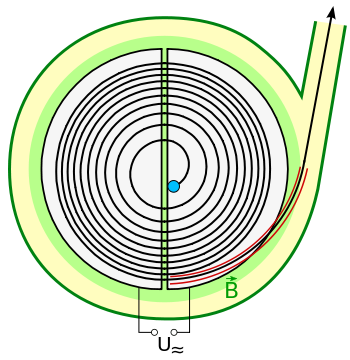
\includegraphics[width=0.35\textwidth]{Zyklotron_Prinzipskizze02.png}
%	\vspace{-13pt}
%	\caption{Prinzipskizze eines Zyklotrons}
%	\vspace{-5pt}	
%	
%\end{wrapfigure}

%\subsubsection{Anwendung}

% Some Formula:

%\begin{equation}
%	x= \frac{y \cdot 13 \pi z}
%			{\cos \alpha}
%\end{equation}

%%%%%%%%%%%%%%%%%%%%%%%
% Eigentlicher Beginn %
%%%%%%%%%%%%%%%%%%%%%%%

\subsection{Prinzip}

Ein Zyklotron besteht aus Zwei hohlen, halbzylindrischen und Duanden an denen eine Spannung mit unterschiedlichem Vorzeichen anliegt, und darüber bzw. darunter liegende Magneten, die ein homogenes Magnetfeld erzeugen. Zudem gibt es einen Einlass und einen Auslass für Teilchen.

%\begin{wrapfigure}{r}{0.4\textwidth} \label{Zyklo}

%	\vspace{-10pt}
%	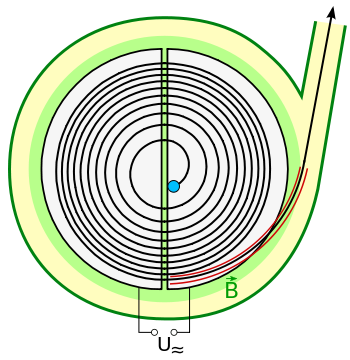
\includegraphics[width=0.35\textwidth]{Zyklotron_Prinzipskizze02.png}
%	\vspace{-13pt}
%	\caption{Prinzipskizze eines Zyklotrons}
%	\vspace{-5pt}	
	
%\end{wrapfigure}

Die Teilchenquelle im Inneren des Zyklotrons setzt Elektronen oder Protonen frei. Diese Teilchen werden durch das Magnetfeld mithilfe der Lorentzkraft auf eine Kreisbahn gezwungen (siehe Sektion \ref{Kreisbahn}). Das Teilchen wird nun zum entgegengesetzt geladenen Duanden gezogen und beschreibt in diesem eine 180%\degree{}
Kurve und sobald es wieder in den Spalt zwischen den Duanden eintritt, werden diese umgepolt, sodass das Teilchen nun zum anderen Duanden gezogen wird. Die Umpolungsfrequenz bleibt über den ganzen Versuch gleich. 

In diesem Spalt wird das Teilchen abermals und abermals beschleunigt bis es aus dem Zyklotron austritt.

\subsection{Gesetze}

\subsubsection{Radius}

Aus der Gleichsetzung der Zentrifugalkraft und der Lorentzkraft ergibt sich: \\

$
F_Zf = F_Lr
$ 

$
\frac{m \cdot v^2}{r} = q_e \cdot v \cdot B
$ \\

\hspace{-7mm} Daher gilt für den Radius:

\begin{equation}
	r = \frac{m_e \cdot v}{B \cdot q_e}
\end{equation}


\subsubsection{Frequenz}

Aus den folgenden Betrachtungen ergibt sich für ein Elektron: \\

$
t = \frac{s}{v} = \frac{2 \pi r}{v} = T
$

$
r = \frac{m_e \cdot v}{q_e \cdot B}
$

$
f = \frac{1}{T} = \frac{v}{2 \pi r}
= \frac{v \cdot q_e \cdot B}{2 \pi \cdot m_e \cdot v} 
= \frac{q_e \cdot B}{2 \pi \cdot m_e}
$ \\

\hspace{-7mm}Daher gilt für die Frequenz:

\begin{equation}
	f = \frac{q_e \cdot B}{2 \pi \cdot m_e}
\end{equation}